\documentclass[11pt,a4paper]{article}
\usepackage[margin=1in]{geometry}
\usepackage{hyperref}
\usepackage{enumitem}
\usepackage{graphicx}
\usepackage{xcolor}
\usepackage{booktabs}
\usepackage{longtable}
\usepackage{array}
\usepackage{float}
\usepackage{tabularx}
\usepackage{titlesec}
\usepackage{titling}
\usepackage[T1]{fontenc}
\usepackage{lmodern}

% -----------------------------------------------------
% Template-compatible helpers
% -----------------------------------------------------
\makeatletter
\newcommand{\BvrSetLabInstructor}[1]{\gdef\Bvr@LabInstructor{#1}}
\newcommand{\Bvr@LabInstructor}{Dr. Raghav B. Venkataramaiyer}
\newcommand{\BvrLabInstructorValue}{\Bvr@LabInstructor}
\makeatother

\pretitle{\begin{center}\bfseries\fontsize{18bp}{18bp}\selectfont}
\makeatletter
\newcommand{\BvrSubtitle}[1]{%
  \posttitle{%
    \par\end{center}
    \begin{center}\large#1\end{center}
    \vskip 0.5em}%
}
\makeatother
\newcommand{\BvrHint}[1]{{\normalfont\normalsize\itshape\hfill #1}}

\title{EcoCode: Green-Software Analysis Platform}
\BvrSetLabInstructor{Dr. Raghav B. Venkataramaiyer}
\BvrSubtitle{%
  Prototype-Stage Project Report for UCS503P \\
  Submitted to: \BvrLabInstructorValue \\ \bfseries
  Thapar Institute of Engineering and Technology
}

\author{%
  Gurnoor Singh Sodhi\thanks{Roll No: \texttt{1024030387}}%
  \and Rakesh\thanks{Roll No: \texttt{1024030393}}%
  \and Manav\thanks{Roll No: \texttt{1024030398}}%
}
\date{September 2026}

\begin{document}
\maketitle
\thispagestyle{empty}
\newpage

\tableofcontents
\newpage

\section{Project Overview}
EcoCode is a deterministic static-analysis prototype for Java projects. Its immediate goal is to identify source-code patterns that may contribute to unnecessary computation, repeated allocation, expensive collection operations, deep call chains, resource-management risks, or other forms of avoidable software resource usage.

The current prototype deliberately focuses on \textbf{whole-project static analysis}. It does not claim that every static finding is a confirmed performance defect. Instead, findings are treated as review candidates whose precision is being improved through testing and false-positive analysis.

\section{Higher-order Goal \BvrHint{green-software framing}}
The higher-order goal is to support more resource-efficient software engineering. EcoCode translates this broad sustainability objective into an engineering problem that can be measured: locate potentially wasteful source-code patterns, attach source-level evidence, and later validate whether recommended changes measurably improve runtime behaviour.

\section{Problem Statement}
Modern Java applications can contain inefficient patterns that are difficult to identify through manual review alone, particularly when projects span many files and classes. Examples include repeated linear lookups inside loops, repeated object allocation on frequently executed paths, resource-management risks, unnecessary duplicate computation, and deep delegation chains.

Existing profilers are useful after software is running, but the team wanted an early-stage engineering tool that can inspect a complete repository before runtime profiling and produce deterministic, explainable findings tied to source files and methods.

\section{Time-to-Value and Iterative Delivery}
EcoCode follows an iterative and incremental development model so that each stage produces a usable engineering increment.

\begin{itemize}[leftmargin=0.7cm]
  \item \textbf{Iteration 1 -- Foundation:} Gradle setup, project indexing, Java file metadata, JavaParser integration, whole-project parsing, ProjectModel.
  \item \textbf{Iteration 2 -- Static Relationships:} method-call extraction, lightweight symbol-resolution layer, call-graph construction, reachability/depth support.
  \item \textbf{Iteration 3 -- Rule Engine:} EcoRule abstraction, RuleEngine, EC101--EC108, JUnit tests, open-source repository validation, false-positive refinement.
  \item \textbf{Next iteration:} build automation and runtime intelligence, including containerized execution and profiling evidence.
\end{itemize}

This structure supports the course emphasis on fast build-test-feedback cycles rather than waiting for a single final implementation.

\section{Current Architecture}
Figure~\ref{fig:architecture} summarizes the current Iteration-3 analysis pipeline.

\begin{figure}[H]
  \centering
  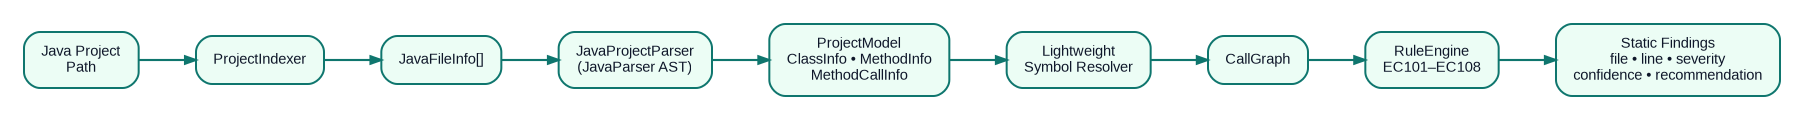
\includegraphics[width=0.95\textwidth]{assets/architecture.png}
  \caption{EcoCode Iteration-3 architecture}
  \label{fig:architecture}
\end{figure}

The active prototype pipeline is:
\begin{center}
Project Path $\rightarrow$ ProjectIndexer $\rightarrow$ JavaProjectParser $\rightarrow$ ProjectModel $\rightarrow$ SymbolSolver $\rightarrow$ CallGraph $\rightarrow$ RuleEngine $\rightarrow$ Static Findings.
\end{center}

The current \texttt{SymbolSolver} is a \textbf{lightweight deterministic resolver}; it should not be described as full JavaParser semantic symbol solving.

\section{Analysis Phase}
\subsection{Use Cases}
The main actor is a developer or evaluator who selects a Java project and requests analysis. EcoCode indexes the repository, parses source files, constructs an internal model, extracts static relationships, executes deterministic rules, and reports source-linked findings.

\begin{figure}[H]
  \centering
  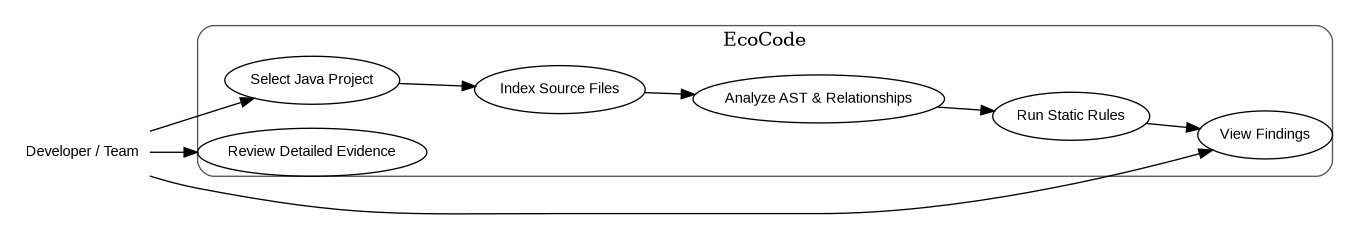
\includegraphics[width=0.90\textwidth]{assets/usecase.png}
  \caption{Use-case diagram}
\end{figure}

\subsection{Activity / Swimlane Diagram}
\begin{figure}[H]
  \centering
  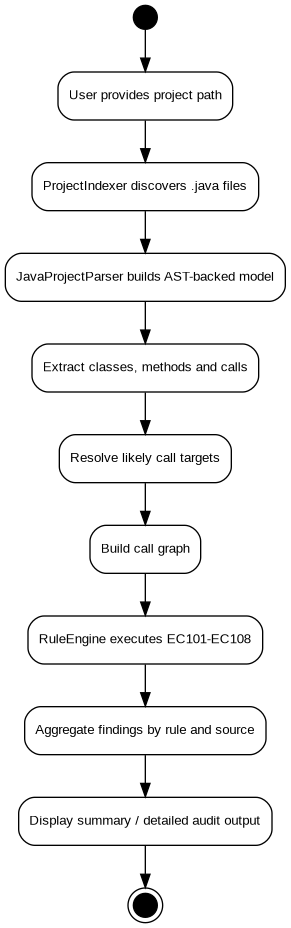
\includegraphics[width=0.95\textwidth]{assets/activity.png}
  \caption{Activity and responsibility flow}
\end{figure}

\subsection{Class Diagram}
\begin{figure}[H]
  \centering
  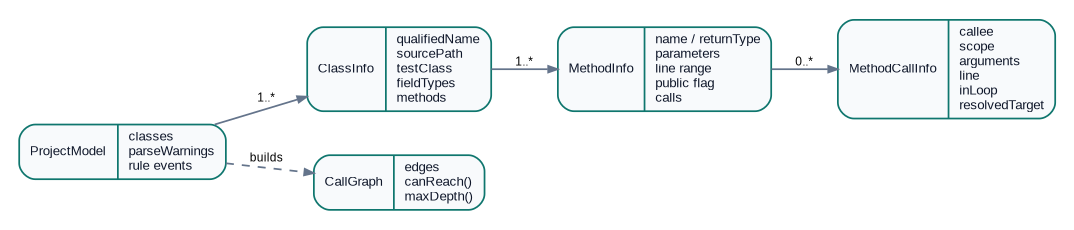
\includegraphics[width=0.98\textwidth]{assets/class_model.png}
  \caption{Core class model for the static-analysis prototype}
\end{figure}

The main classes include \texttt{ProjectIndexer}, \texttt{JavaFileInfo}, \texttt{JavaProjectParser}, \texttt{ProjectModel}, \texttt{ClassInfo}, \texttt{MethodInfo}, \texttt{MethodCallInfo}, \texttt{SymbolSolver}, \texttt{CallGraph}, \texttt{EcoRule}, \texttt{RuleEngine}, the eight EC rules, and \texttt{StaticIssue}.

\subsection{Data Flow Diagrams}
\subsubsection{DFD Level 0}
\begin{figure}[H]
  \centering
  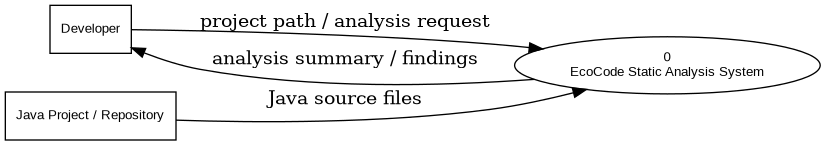
\includegraphics[width=0.90\textwidth]{assets/dfd0.png}
  \caption{DFD Level 0}
\end{figure}

\subsubsection{DFD Level 1}
\begin{figure}[H]
  \centering
  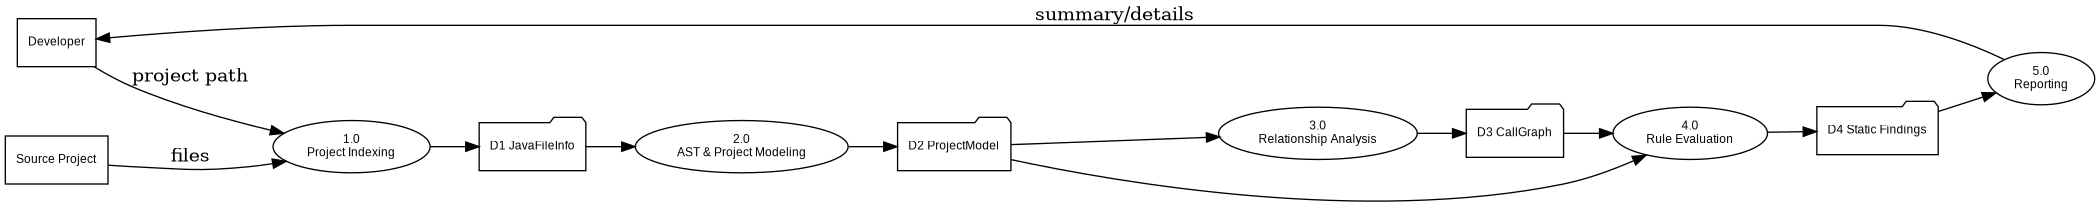
\includegraphics[width=0.95\textwidth]{assets/dfd1.png}
  \caption{DFD Level 1}
\end{figure}

\subsubsection{DFD Level 2}
\begin{figure}[H]
  \centering
  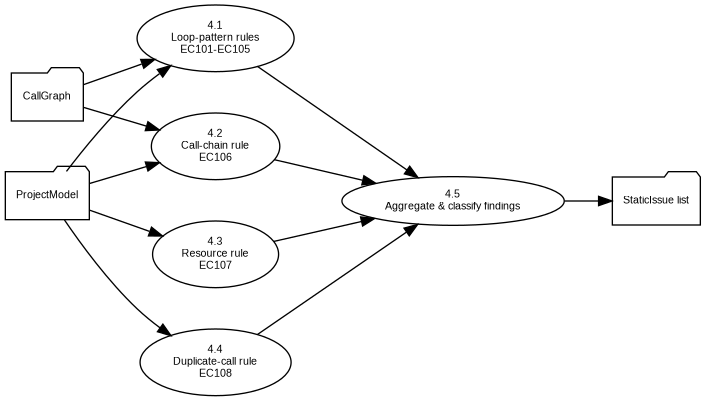
\includegraphics[width=0.95\textwidth]{assets/dfd2.png}
  \caption{DFD Level 2}
\end{figure}

\section{Software Requirement Specification \BvrHint{IEEE-style}}
\subsection{Purpose}
The purpose of EcoCode is to analyse complete Java projects and produce deterministic, explainable static findings that may indicate opportunities for resource-efficiency improvement.

\subsection{Scope}
The prototype currently supports local Java-project analysis. It indexes source files, parses Java source into ASTs, builds a project model, extracts method calls, constructs a prototype call graph, and applies EC101--EC108. Runtime profiling, evidence confirmation, version comparison, and production deployment are future-stage features.

\subsection{Functional Requirements}
\begin{longtable}{p{0.12\textwidth}p{0.80\textwidth}}
\toprule
\textbf{ID} & \textbf{Requirement} \\
\midrule
FR1 & The system shall accept a local Java project path as input. \\
FR2 & The system shall recursively identify Java source files. \\
FR3 & The system shall record file metadata including line count and test/non-test classification. \\
FR4 & The system shall parse Java source files and build a whole-project model. \\
FR5 & The system shall extract classes, methods, method calls, and source locations. \\
FR6 & The system shall apply a lightweight deterministic symbol-resolution layer. \\
FR7 & The system shall construct a prototype call graph from extracted method relationships. \\
FR8 & The system shall execute EC101--EC108 through a common rule-engine abstraction. \\
FR9 & The system shall report rule ID, file, line, class, method, severity/confidence, explanation, and recommendation where available. \\
FR10 & The system shall distinguish test-code findings from non-test source findings. \\
\bottomrule
\end{longtable}

\subsection{Non-Functional Requirements}
\begin{itemize}[leftmargin=0.7cm]
  \item \textbf{Explainability:} Findings should be deterministic and source-linked.
  \item \textbf{Maintainability:} Rules should implement a shared abstraction so they can be refined independently.
  \item \textbf{Scalability:} The architecture should extend from small repositories to larger multi-file Java projects.
  \item \textbf{Reproducibility:} The same source tree and rule version should produce repeatable static findings.
  \item \textbf{Portability:} The prototype targets Java 21 and Gradle-based execution.
\end{itemize}

\section{Rule Engine}
The current rule set is shown below. These rules are implemented but are \textbf{still under testing}; their thresholds and false-positive behaviour are not considered final.

\begin{table}[H]
\centering
\small
\begin{tabularx}{\textwidth}{>{\bfseries}p{0.12\textwidth}X}
\toprule
Rule & Current interpretation \\
\midrule
EC101 & Repeated database/repository call in a loop \\
EC102 & Accumulating string concatenation in a loop \\
EC103 & Linear collection lookup in a loop \\
EC104 & Potential unbounded collection fetch \\
EC105 & Potential repeated object allocation in a loop \\
EC106 & Deep call-chain review signal \\
EC107 & Potential unclosed system resource \\
EC108 & Potential duplicate computation \\
\bottomrule
\end{tabularx}
\end{table}

\section{Prototype Validation}
The current reference repository is \texttt{minimal-json}. The latest validated run produced the following structural metrics:

\begin{table}[H]
\centering
\begin{tabular}{lr}
\toprule
Metric & Result \\
\midrule
Java files & 54 \\
Non-test source files & 37 \\
Test files & 17 \\
Lines of code & 10,870 \\
Classes & 63 \\
Methods & 912 \\
Method calls & 2,931 \\
Call-graph nodes & 468 \\
Parse warnings & 0 \\
Static findings & 106 \\
Non-test source findings & 42 \\
Test-code findings & 64 \\
\bottomrule
\end{tabular}
\end{table}

\subsection{Rule Counts on the Reference Run}
\begin{table}[H]
\centering
\small
\begin{tabular}{lrr}
\toprule
Rule & Total & Non-test source \\
\midrule
EC101 & 0 & 0 \\
EC102 & 0 & 0 \\
EC103 & 4 & 4 \\
EC104 & 0 & 0 \\
EC105 & 20 & 13 \\
EC106 & 1 & 1 \\
EC107 & 14 & 5 \\
EC108 & 67 & 19 \\
\bottomrule
\end{tabular}
\end{table}

The team initially observed 285 findings before auditing the heuristics. Manual review exposed broad interpretations in some rules, and the rules were made more conservative. The latest reference run reports 106 findings. This reduction is treated as evidence of \textbf{false-positive refinement}, not as loss of functionality.

\section{Evaluation Criterion}
At the prototype stage, success is evaluated using measurable engineering evidence:
\begin{itemize}[leftmargin=0.7cm]
  \item complete parsing of the selected repository with zero parser warnings on the reference run;
  \item reproducible structural metrics (files, LOC, classes, methods, calls, graph nodes);
  \item automated JUnit tests for rule behaviour;
  \item manual inspection of representative findings;
  \item reduction of demonstrable false positives while preserving intended detections.
\end{itemize}

Later evaluation will include runtime measurements so potential findings can be confirmed or rejected with evidence.

\section{User Stories and Story Cards}
\begin{itemize}[leftmargin=0.7cm]
  \item \textbf{US1:} As a developer, I want to scan an entire Java repository so that I can review potential resource-efficiency issues without inspecting every file manually.
  \item \textbf{US2:} As a developer, I want each finding to include a rule ID, source file, method, and line so that I can verify the evidence quickly.
  \item \textbf{US3:} As a maintainer, I want rules to use a shared interface so that rules can be added, tested, or refined independently.
  \item \textbf{US4:} As an evaluator, I want project-level metrics and parse warnings so that I can judge whether the analyser actually processed the repository.
  \item \textbf{US5:} As a developer, I want test-code findings separated from non-test source findings so that analysis results are easier to interpret.
\end{itemize}

\section{SDLC Model}
EcoCode uses an \textbf{Agile Iterative and Incremental} model. Each iteration produces a working increment, is tested on real code, and feeds observed problems back into the next increment. This model is suitable because static-analysis heuristics improve through repeated build-test-review cycles rather than a single one-time implementation.

\section{Current Limitations}
\begin{itemize}[leftmargin=0.7cm]
  \item Rule testing and false-positive refinement are ongoing; rules are not finalised.
  \item Static findings are not equivalent to confirmed performance defects.
  \item The current symbol resolver is heuristic rather than full semantic JavaParser Symbol Solver integration.
  \item EC105, EC106, EC107, and EC108 are intentionally conservative review signals in the prototype.
  \item Runtime profiling and evidence confirmation are not part of the current Iteration-3 submission.
\end{itemize}

\section{Next Iteration}
The next planned stream moves from static intelligence toward runtime evidence: build automation, containerized execution, benchmark management, JVM profiling, and an evidence layer that can classify static findings as potential, confirmed, validated, or rejected.

\section{Team Contribution Summary}
\begin{itemize}[leftmargin=0.7cm]
  \item \textbf{Gurnoor Singh Sodhi:} static-analysis foundation, project indexing, JavaParser/project-model work, integration understanding, rule validation and false-positive audit, documentation and presentation preparation.
  \item \textbf{Rakesh:} runtime-intelligence stream ownership including build execution, Docker/runtime profiling, benchmark and system-metric work according to the team roadmap.
  \item \textbf{Manav:} integration/validation stream, version comparison, repository integration, UI/backend integration and testing according to the team roadmap.
\end{itemize}

\section{Conclusion}
EcoCode has reached a working Iteration-3 static-analysis prototype. It can process a real multi-file Java repository, build structural and call-relationship information, execute a deterministic eight-rule engine, and report source-linked findings. The team is deliberately presenting the rule set as \textbf{implemented but still under validation}. The next stage will add runtime evidence so the system can move from potential static patterns toward measurable green-software recommendations.

\end{document}
